%------------------------------------------------------------------------
% Chapter:  PDF calculation
%------------------------------------------------------------------------

\chapter{Atomic pair distribution function \label{pdf}}

The atomic pair distribution function (PDF) can be obtained from
powder diffraction data and is a valuable tools for the study of the
{\it local} atomic arrangements in a material. This chapter
describes how \Discus can be used to calculate and refine a
PDF. It might be interesting to know about the existence of the
program {\it PDFFIT} \citep{prbi99} which allows the full profile
structural least square refinement of a PDF. {\it PDFFIT} uses a
command language and structure file format similar to \Discus
and can be obtained from the same source. The PDF of a given
structure can be calculated using the relation:
%
\begin{equation}
  G_{c}(r) = \frac{1}{r} \sum_{i}\sum_{j} \left [
             \frac{b_{i}b_{j}}{\langle b \rangle ^{2}}
             \delta (r - r_{ij}) \right ]   - 4 \pi r \rho_{0},
  \label{eq_igr}
\end{equation}
%
where the sum goes over all pairs of atoms $i$ and $j$ within the
model crystal separated by $r_{ij}$. The scattering power of atom
$i$ is $b_{i}$ and $\langle b \rangle$ is the average scattering
power of the sample. In case of neutron scattering $b_{i}$ is simply
the scattering length, in case of X-rays it is the atomic form
factor evaluated at a user define value of $Q$. The default value is
$Q=0$ in which case $b_{i}$ is simply the number of electrons of
atom $i$. Generally there are two different ways to account for
displacements (either thermal or static) from the average position.
First one can use a large enough model containing the desired
displacements and perform an ensemble average. Secondly one can
convolute each contribution given by $\delta (r - r_{ij})$ in
(\ref{eq_igr}) with a Gaussian accounting for the displacements.
Alternatively, the PDF peak width can be approximated by the ensemble
average of a distorted structure. \par

As we have seen before, the experimental PDF is obtained by
Fourier transform of the reduced structure factor. However, the
accessible range in $Q$ is limited by $Q_{max}$. This can be
described by a multiplication of the structure factor up to
infinity with a step function cutting off at $Q=Q_{max}$ resulting
in the convolution of the PDF with the Fourier transform  $S(r)$
of the step function. \Discus models the finite $Q$-range by
convoluting the model PDF $G(r)$ with
%
\begin{equation}
  S(r) = \frac{\sin(Q_{max} \cdot r)}{r}
  \label{eq_sinc}
\end{equation}
%
One last correction applied to the calculated PDF, $G_{c}(r)$,
accounts for the limited resolution of the experiment in $Q$-space.
This leads to a decrease of the PDF peak as a function of $r$
according to the relation $\exp(-\sigma_{Q}^{2}r^{2}/2)$. A detailed
discussion of the accuracy of PDF analysis is given in
\citet{toeg92}. More examples and exercises related to the PDF
calculation in \Discus are in our cookbook \citep{nedpro}.

%------------------------------------------------------------------------

\section{Calculating the PDF \label{pdf-calc}}

The calculated PDF for Nickel is shown in figure \ref{pdf-fig1}.
The PDF was calculated for two different situations: The PDF shown
as dotted line was calculated without applying convolution given
by $Q_{max}$. This is achieved in \Discus by setting the
value of $Q_{max}$ to zero. The second PDF shown as solid line in
figure \ref{pdf-fig1} was calculated for $Q_{max} = 20$\AA$^{-1}$.
The resulting termination ripples are clearly visible.
%
\begin{figure}[!b]
   \centering
   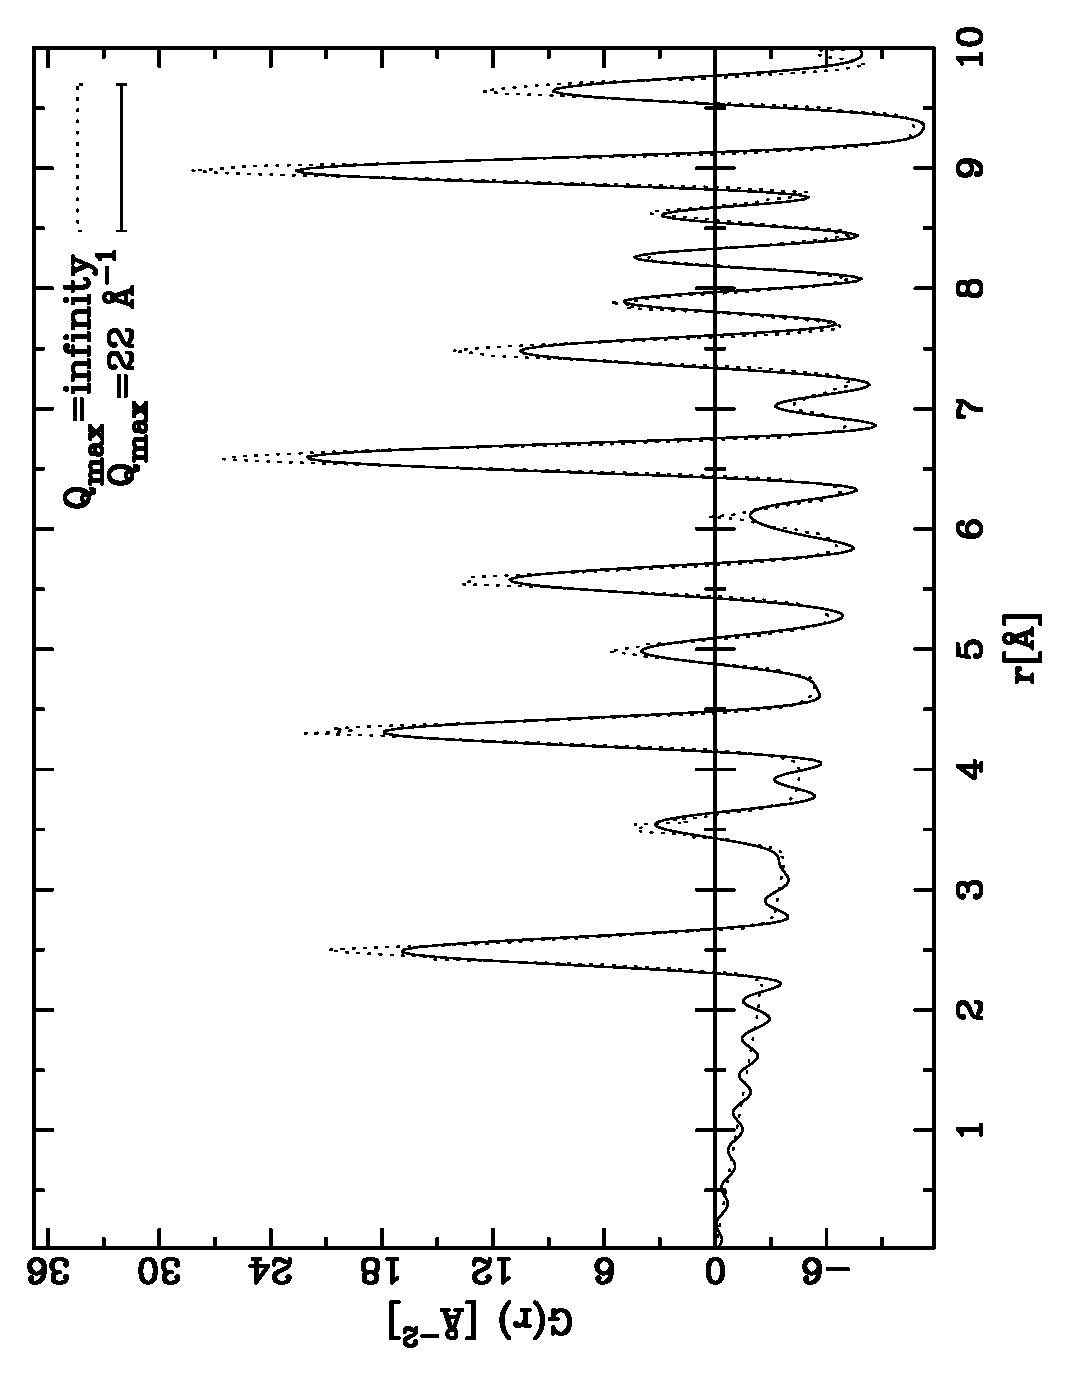
\includegraphics[scale=0.5, angle=270]{pdf.1.eps}
   \caption{Calculated PDFs of $Ni$}
   \label{pdf-fig1}
\end{figure}
%

\begin{MacVerbatim}
      1 read
      2 cell ni.cll,5,5,5
      3 #
      4 therm
      5 #
      6 pdf
      7   set rang,10.0,0.02
      8   set qmax,20.0
      9   set qdamp,0.0
     10   set rad,xray
     11 #
     12   calc
     13 #
     14   save pdf,ni.pdf
     15 exit
\end{MacVerbatim}
%
The macro file used to calculate the Nickel PDFs is listed above.
First we read the unit cell for Nickel and expand it to a size of
5x5x5 unit cells (lines 1--2). Next we introduce thermal vibrations
according to the given isotropic Debye-Waller factor (line 4). After
entering the PDF sub level (line 6) we specify the maximum value of
$r$ and grid size $\Delta r$ (line 7). In our case we calculate up
to a value of $r=10$\AA\ using a grid of $\Delta r=0.02$\AA. The
next command (line 8) specifies the value of $Q_{max}$ to be set to
20\AA$^{-1}$. Finally we set dampening term $\sigma_{Q}$ to 
zero (line 9) meaning
no Q-resolution correction and select X-ray radiation (line 10). Now
we are ready to calculate the PDF, done in line 12. All we have to
do now is to save the result to a file (line 14). The result is
shown in figure \ref{pdf-fig1}. \par

When discussing equation (\ref{eq_igr}) used to calculate the PDF
from a structural model, we just stated that the sum over $ij$ goes
over {\it all} pairs of atoms $i$ and $j$ within the model crystal.
This is perfectly correct to calculate a total PDF. However
sometimes it might be desired to calculate just a partial or
differential PDF. by selecting the elements of interest.

%------------------------------------------------------------------------

\section{Refining a PDF \label{pdf-rmc}}

In principle an experimental PDF can be refined based on a
structural model in two different ways. A relatively small model can
be refined using {\it PDFFIT}. On the other hand a larger model can
be refined using the Reverse Monte Carlo (RMC) algorithm in 
\discus. Details about the principle of RMC are discussed in chapter
\ref{rmc} of this manual. The only difference is that rather than
refining the scattering intensity directly, the PDF is refined. An
example refinement of a Nickel PDF is listed below and is also part
of the online tutorial of \discus.
%

\begin{MacVerbatim}
      1 read
      2 cell ni.stru
      3 #
      4 pdf
      5   data ni.data
      6 #
      7   set frange,1.5,10.0
      8   set qmax,22.0
      9   set rad,xray
     10   sel ni
     11   set mode,shift
     12   set move,ni,0.01,0.01,0.01
     13   set disp,1
     14   set cyc,25
     15   show all
     16   run
     17   save pdf,rmc.pdf
     18   save stru,rmc.stru
     19 exit
\end{MacVerbatim}
%
In lines 1--2 the starting structure is read. Next the {\tt pdf}
sub level is entered (line 4). First we read the observed PDF from
the file {\it ni.data}. The maximum $r$ and $\Delta r$ which defines
the range of the calculated PDF are taken from the data file just
read. Then the range in $r$ that actually should be used for the
refinement is set (line 7), here from 1.5 to 10.0\AA. In lines 8--9
the value of $Q_{max}$ and the radiation used in the experiment is
set. Now we enter the RMC related settings (see also \ref{rmc}). We
select atoms to be moved (line 10), here Ni. This command should not
be confused with {\tt isel} or {\tt jsel} which actually selects the
atoms that are included in the calculation of the PDF. The RMC mode
is set to shift atoms using a Gaussian distribution with a sigma of
0.01 lattice units ($\approx 0.035$\AA) in lines 11--12. Finally we
set the screen update interval to 1 (line 13) and specify that 25
cycles will be carried out (line 14). Before the refinement is
started in line 16, the current settings are displayed using the
command {\tt show} (line 15). After the refinement is finished, the
resulting PDF (line 17) and structure (line 18) is saved to a file.
\par

%------------------------------------------------------------------------
